
% !TEX TS-program = pdflatex
% !TEX encoding = UTF-8 Unicode

% This is a simple template for a LaTeX document using the "article" class.
% See "book", "report", "letter" for other types of document.

\documentclass[11pt]{article} % use larger type; default would be 10pt

\usepackage[utf8]{inputenc} % set input encoding (not needed with XeLaTeX)

%%% Examples of Article customizations
% These packages are optional, depending whether you want the features they provide.
% See the LaTeX Companion or other references for full information.

%%% PAGE DIMENSIONS
\usepackage{geometry} % to change the page dimensions
\geometry{a4paper} % or letterpaper (US) or a5paper or....
% \geometry{margin=2in} % for example, change the margins to 2 inches all round
% \geometry{landscape} % set up the page for landscape
%   read geometry.pdf for detailed page layout information

\usepackage{graphicx} % support the \includegraphics command and options

% \usepackage[parfill]{parskip} % Activate to begin paragraphs with an empty line rather than an indent

%%% PACKAGES
\usepackage{booktabs} % for much better looking tables
\usepackage{array} % for better arrays (eg matrices) in maths
\usepackage{paralist} % very flexible & customisable lists (eg. enumerate/itemize, etc.)
\usepackage{verbatim} % adds environment for commenting out blocks of text & for better verbatim
\usepackage{subfig} % make it possible to include more than one captioned figure/table in a single float
% These packages are all incorporated in the memoir class to one degree or another...

%%% HEADERS & FOOTERS
\usepackage{fancyhdr} % This should be set AFTER setting up the page geometry
\pagestyle{fancy} % options: empty , plain , fancy
\renewcommand{\headrulewidth}{0pt} % customise the layout...
\lhead{}\chead{}\rhead{}
\lfoot{}\cfoot{\thepage}\rfoot{}

%%% SECTION TITLE APPEARANCE
\usepackage{sectsty}
\allsectionsfont{\sffamily\mdseries\upshape} % (See the fntguide.pdf for font help)
% (This matches ConTeXt defaults)

%%% ToC (table of contents) APPEARANCE
\usepackage[nottoc,notlof,notlot]{tocbibind} % Put the bibliography in the ToC
\usepackage[titles,subfigure]{tocloft} % Alter the style of the Table of Contents
\renewcommand{\cftsecfont}{\rmfamily\mdseries\upshape}
\renewcommand{\cftsecpagefont}{\rmfamily\mdseries\upshape} % No bold!

\makeatletter
   \newcommand\figcaption{\def\@captype{figure}\caption}
   \newcommand\tabcaption{\def\@captype{table}\caption}
\makeatother
%%% END Article customizations

%%% The "real" document content comes below...

\title{CSE 509 Lecture 22}

\author{Prof. Rob Johnson, Scribe:Arun Rathakrishnan}
%\date{} % Activate to display a given date or no date (if empty),
         % otherwise the current date is printed 

\begin{document}
\maketitle
\section {Native Client Applications}
Native Client is a mechanism for  an application to run untrusted code in its
address space. There are several situtations in which untrusted code has to be
executed by an application. Network Packet filters require the kernel execute
some untrusted code in the kernel space. Plugins supported by web browsers also
fall in this category. In Google Chrome, the plugin is executed as a separate
process so that, the browser process is isolated from the untrusted plugin code.
The aim is to protect the untrusted code from adversely affecting the target
application and prevent it from stealing sensitive information.\\

The isolated processes communicate through Inter Process Communication. But if the
interaction between processes is high, there is a huge communication overhead
due to IPC. This overhead can be avoided, if untrusted code runs in the same
address space as the application,
\begin {itemize} \itemsep -2pt
\item but is prevented from accessing some parts of the application's resources
such as code section, stack, heap, etc.
\item The native client must not be allowed to make arbitrary system calls.
\end {itemize}.
If we can enforce the above restrictions, the untrusted code can execute in the 
same process as the application reducing the communication costs due to IPC.
\section {Inline Reference Monitors}
When native code executes in the target application, the below conditions must
hold.
\begin {description} \itemsep -2pt
\item [Memory Isolation] Restrict untrusted component to only
read or write its own memory.
\item [Control Privileged Actions] Prevent system calls and
ensure the code runs in user mode.
\item [Cross Domain Calls] Communicate with the target application.
Application needs to make calls to the native code and native code may make use
of libraries that are part of the application's address space.
\end {description}
A compiler for native clients can perform binary instrumentation by,
\begin {itemize} \itemsep -2pt
\item Inserting run-time checks into the untrusted binary. Check if memory
references are safe.
\item Preventing bad jumps, that bypass these checks.
\item Verify correctness of the compilation.
\end {itemize}
\subsection {Verification Process}
\begin {center}
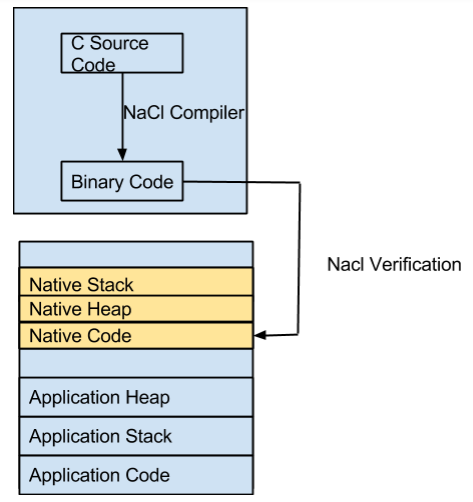
\includegraphics [width=390px,height=460px]{img/f1.png} \\
\caption {Compilation, Verification and Memory Organization}
\end {center}
\pagebreak
\subsection {Organization}
A separate compiler is required for compiling applications that support native
clients. The untrusted code is confined to a separate memory region within the 
process address space that supports stack, heap and code section that are isolated
from the application's. When the control goes to native code, we track all memory
references and ensure that they are within the bounds of the isolated memory region.
\subsection {Bounds Checking}
One strategy is to use two registers to store the bounds of the isolated memory
region. Before any memory access we need to check if the address is within bounds.
In the example below, we consider the execution of a load instruction in a $64$
bit machine.
\begin {verbatim}
load [%r0], %r1
\end {verbatim}

\begin {verbatim}
bl %r0, %r14, .ERR
bl %r15, %r0, .ERR
\end {verbatim}
\\By aligning the isolated memory region to power of 2 boundaries, we can reduce
the number of registers used or the number of instructions required for the check.
When the control is with the untrusted code PC value will always remain within the
$2^k$ range. By making use of the fact we know $k$ and can force any memory 
access to be within the untrusted region.
\begin {verbatim}
shr %pc, k, %r2
shl %r0, 64-k, %r0
shr %r0, 64-k, %r0
or %r2, %r1
\end {verbatim}
Even if the address is outside the range, it is forced to be within the memory
range.  This is called pointer swizzling. Since we only care about confining the
memory access in the untrusted region, this is a valid approach. 
\subsection {Preventing Bad Jumps}
Once the bounds checking instructions are in place, we must ensure that the native
binary does not have a way to get around this. The only way to prevent the execution
of such instructions is to insert jump instructions so that the machine jumps over
bounds checking code and performs illegal memory accesses.\\

Jump instructions come in three flavours.
\begin {itemize} \itemsep -2pt
\item jmp direct address
\item jmp \%pc + offset
\item jmp \%r0
\end {itemize}
The first two types can be verified by static checking to see if they skip bounds
checking. The third type of jump occurs during in switch case statements and
can be resolved only during the runtime. This is performed by the same bounds
check on address in register's contents. But this alone is not sufficient to 
ensure that no bounds instruction is skipped. \\

However there is a simple trick that is sufficient. We organize the binary 
instructions, so that the bounds check code always start at $32$ byte boundaries.
As result, if the original instruction to be executed after jump is a memory access
we are sure that bounds checking instructions will be at the next instruction to
which the control transfers to.\\

Given the native binary, we must disassemble the binary to get byte code, which is
later instrumented with boundary conditions, that start at 32 byte boundaries. The
instrumented code must satisfy the following conditions to prevent illegal access
by the untrusted code.
\begin {itemize} \itemsep -2pt
\item All jumps are to  0 mod 32.
\item All jumps are bounds checked.
\item All loads/stores are bounds checked.
\item No instruction stradles the $32$ byte boundary. We can pad using nops to 
achieve this.
\item Bound check instruction must be within the same $32$ byte range as the
memory access instruction and must begin at the boundary of the region.
\end {itemize}
\\A linear sweep disassembler can convert the native application binary to byte
code, that can be executed within the address space of the target application.
\end{document}

